\chapter{Introduction\label{cha:introduction}}
%% \ifdraft only shows the text in the first argument if you are in draft mode.
%% These directions will disappear in other modes.
%\textit{\ifdraft{State the objectives of the exercise. Ask yourself:
 % \underline{Why} did I design/create the item? What did I aim to achieve? What is the problem I am trying to solve?  How is my solution interesting or novel?}{}}
  %% Using a robot to generate training data for previously unseen objects

A robot is a machine that is often used to do human work in a much more precise and efficient way than the human himself and in more difficult situations. Robots can increase flexibility in the production environment by assisting in a working area. One of the benefits is that robots have high accuracy and can handle heavy and dangerous objects. Robots can be a good replacement for current human labor and can easily replace staff. As a result, increased efficiency due to robotics will boost worker well-being by increasing wages and providing more leisure time.

Picking unseen items is a required skill for robots to learn, it enables them to achieve more general-purpose usefulness. To visually find the best picking point for a given object, such general-purpose robots can use their perception abilities.

To compare this process with human beings, it can be pointed out that it takes a child around 3-6 months to achieve good eyesight on an object and coordinate it. Then it can take around 6-12 months for the child to be able to choose an object, knowing what it is, and know-how to pick it up. It is therefore interesting to see how long it will take a robot with the help of a computer vision to learn these things and pick up an unseen object. 

For a robot to pick up unseen objects\cite{xie_unseen_2021} the robot would need to look at the object, find outlines of the object, a flat surface, and find the center point of the object by using an existing neural network. Assuming the robot has a single point of view of a bin filled with unseen items. When the center point has been found the robot can pick up the object with a suction cup. The robot would then need to place the object in a new place in the bin and take a new photo and train the neural network. However, a part of the problem is to determine suitable methods for picking, arranging, and labelling. The object detection would be done using methods of deep learning. This process is intended to reduce the manual registration effort associated with introducing new objects for automatic picking and packing


The main objective for this project is therefore to use a robot manipulator to generate training data for previously unseen objects. 
Three smaller objectives will be considered in this project. 
First, generate new arrangements of objects using a robot manipulator to train a network to handle the new objects.  
Second, to create object labels by automatically determining the size of the objects in the images.
The third one is to measure the accuracy of object detection using a deep neural network trained on the robot-generated data.
% koma meira inná segja hvað á að gera.... 

The project was divided into three main parts which can been seen in \textit{Figure \ref{fig:project}} and were: \textit{controlling the robot}, \textit{using the camera to find objects} and \textit{use labelled images to train a neural network}. 
\begin{figure}[h]
    \centering
    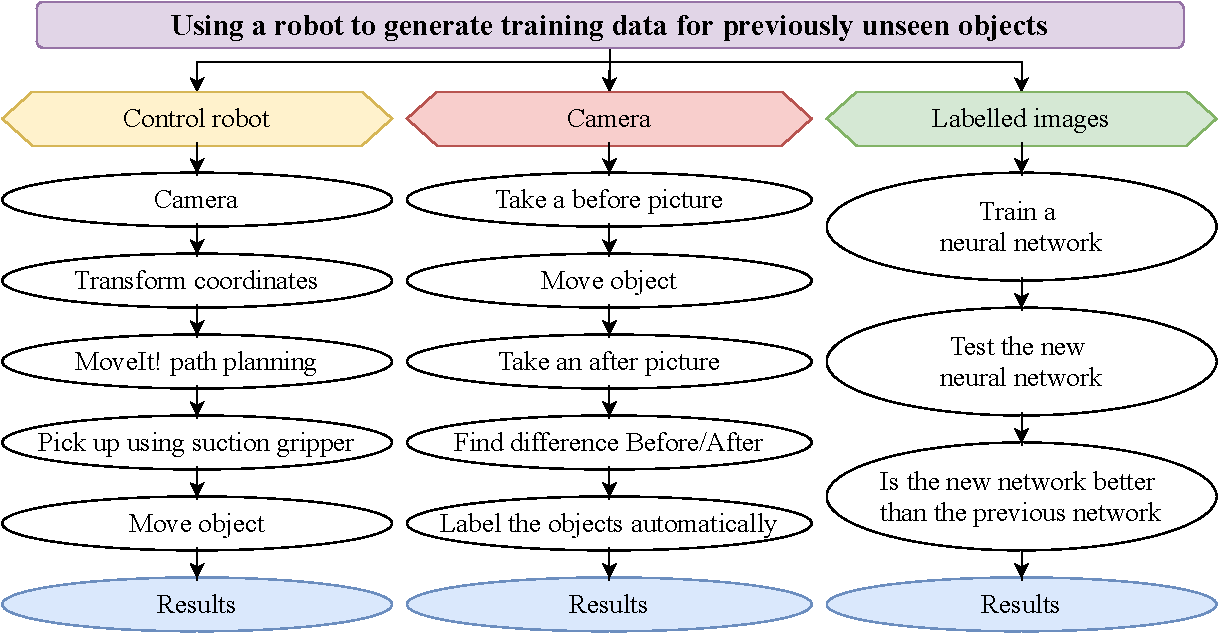
\includegraphics[width=1\textwidth]{graphics/meis.pdf}
    \caption{An flowchart that shows how the project is divided}
    \label{fig:project}
\end{figure}


\section{Background}
% \ifdraft{Provide background about the subject matter (e.g. How was morse code
% developed?  How is it used today?). 
% This is a place where there are usually many citations.
% It is suspicious when there is not.
% Include the purpose of the different equipment and your design intent. 
% Include references to relevant scientific/technical work and books.
% What other examples of similar designs exist?
% How is your approach distinctive?

% If you have specifications or related standards, these must be
% described and cited also.  As an example, you might cite the specific
% RoboSub competition website (and documents) if working on the lighting system for an AUV%\cite{guls2016auvlight}

% %% Glossary is broken, do not use --foley
% % \gls{auv}\footnote{Autonomous Undersea Vehicle}.

% % Notice that there is now information on the AUV in the Index and Acronyms.
% % It isn't in the \gls{glossary} because we didn't put it there.
% % \index{AUV}
% }{}

\subsection{Bin picking}\label{sec:binpicking}
Since the development of the first industrial robot, the automation of handling tasks has been an important scientific topic. In this context, one of the examples is the so-called “bin picking” problem\cite{buchholz_bin-picking_2015}. 
For humans, it is an easy task to pick up objects in a box, but it can be a very complex task for robots. 
Bin picking contains several subsections, including, scene analysis, object recognition, object localization, grasp planning, and path planning. 
Besides, robots must be able to grasp objects in an infinite number of directions and reach deep into the corners of the bin, at the same time avoiding collisions \cite{truebenbach_is_2019}.

Bin picking can be divided into three categories: \textit{Structured bin picking}, \textit{Semi-structured Bin picking}, and \textit{Random Bin picking}. The main difference between those categories is the difficulty level. In \textit{Structured bin picking} objects are placed in an organized pattern so that they can be identified and picked up effortlessly. In \textit{Semi-structured Bin picking} objects are placed with some organization to make picking easier. Finally, in the \textit{Random Bin picking}, objects have completely random positions, multiple directions, and can also overlap each other \cite{noauthor_robotworx_nodate}.

For the bin picking to be fully automated it requires many technologies to work together. Including, a 3D model of the object, the bin, the robot end effector, the placement. Also, a model of ways to pick up the objects with the end effector and deposit it at the placement target. A 3D sensor to map the bin, image analysis software to locate each object and obstacles in the bin, path planning software to avoid collisions. Finally, a robot control software to maneuver the robot \cite{truebenbach_is_2019}.


In the setup and programming, there does the teaching takes place e.g. how to pick up an object, where to put it down, obstacles to avoid, etc. Path planning is another important task for system reliability, but this task is outside the scope of this thesis. 
To plan a unique, collision-free path for each object in the bin to the placement target. Path planning is the main determinant of system reliability because if it is not done well enough the objects can be dropped, left out in the bin, or missed targets and there can be collisions \cite{zeng_robotic_2019}.




\subsection{Computer Vision}
%% Úr bók A Guided Tour of computer vision.
The automatic deduction of the structure and properties of a possible complex three-dimensional universe from either a single or several two-dimensional representations of the world is known as computer vision or image comprehension\cite{nalwa_what_1993}. 
Computer vision (CV) is used to deduce the structure and properties of the three-dimensional universe, which include not only geometric properties but also material properties and the lighting of the world. 
The lightness or darkness of surfaces, their colors, textures, and material compositions are examples of geometric properties. Whereas the forms, sizes, and locations of objects are examples of material properties\cite{szeliski_computer_2010}. % úr bók af bókasafni

CV is an artificial intelligence-assisted paradigm that uses cameras, videos, and deep-learning methods to detect the digital world. Parallel to this, CV researchers have been working on mathematical methods for restoring the three-dimensional form and appearance of objects in images\cite{guo_lossy_2018}. 
Designers now have effective methods for constructing a partial 3D model of an area from thousands of partially overlapping images. Designers can construct accurate dense 3D surface models using stereo matching if they have a wide enough collection of views of a particular object or facade\cite{liu_detection_2020}. 
It also entails the development of specific technologies like image recognition, visual recognition, and facial recognition. Mostly, CV is used to achieve high-level understanding of digital processing. The task of CV is to capture, examine, and recognize digital objects and extracts in higher dimensions\cite{manogaran_wearable_2019}.
%Designers can also follow a person's movements with a complex background. 

% \textbf{It is also possible to use a combination of face, clothes, and hair identification and recognition, to find and name all of the people in an image with moderate success. }\fxfatal{ÞARF AÐ LAGA Reference to old}

% \begin{figure}[ht]
%     \centering
%     % include first image
%     \subfloat[]{\includegraphics[width=0.2\textwidth]{graphics/compa.PNG}}
%     \hfill
%     %\subfloat[]{\includegraphics[width=0.2    \textwidth]{graphics/compb.PNG}}
%     %\hfill
%     \subfloat[]{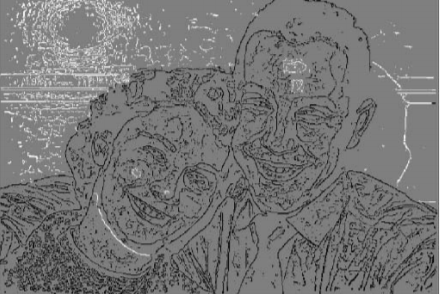
\includegraphics[width=0.2\textwidth]{graphics/compc.PNG}}
%     \hfill
%     \subfloat[]{\includegraphics[width=0.2\textwidth]{graphics/compd.PNG}}
%     \caption{fddsa}
%     \label{figure: computervision}
% \end{figure}
\begin{figure}[ht]
    \centering
    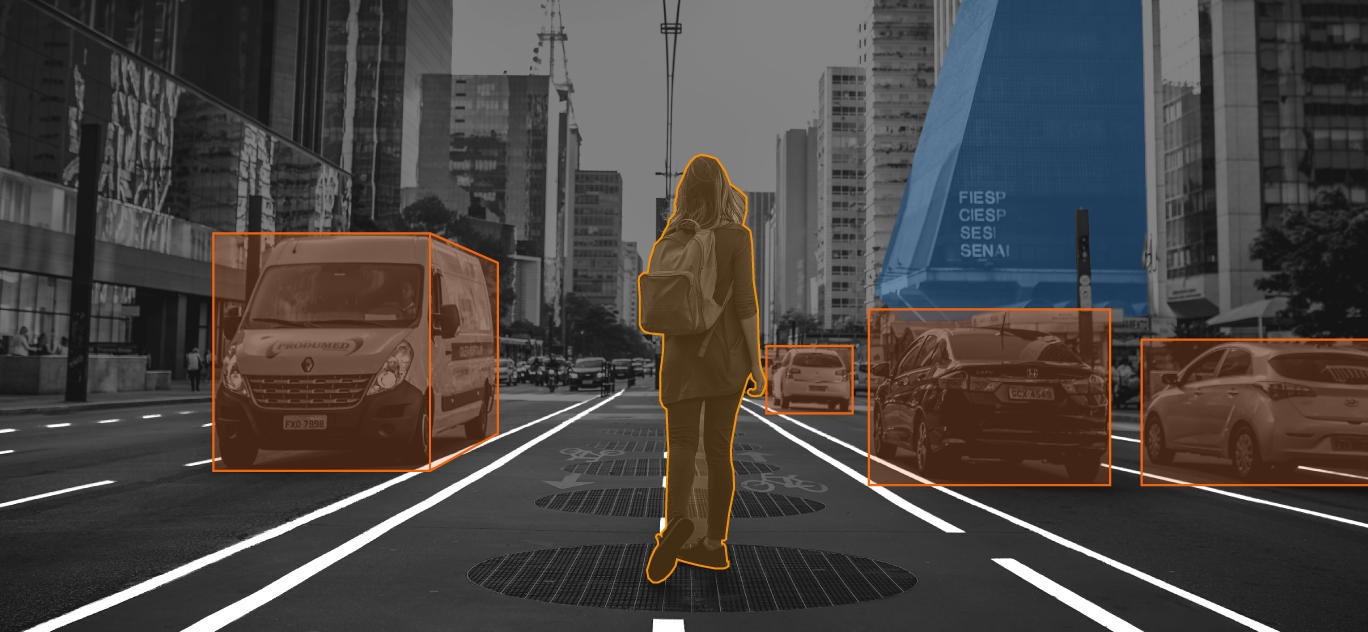
\includegraphics[width=0.85\textwidth]{graphics/mask.png}
    \caption{Computer vision plays a huge role in artificial intelligence, this is a example of a image that has been masked before using as a training data in a neural network  \cite{ambalina_5_2020}}
    \label{fig:mask}
\end{figure}

Computer vision is a branch of computer science that aims to replicate aspects of the complexity of the human vision system, allowing computers to recognize and process objects in images and videos in the same way that human eyes do. Pattern recognition is at the heart of computer vision. One method of teaching a computer to understand visual data is to feed it thousands of images, if not millions, of labeled images. Then subject the images to various software techniques, or algorithms, that allow the computer to search for patterns in all the elements that relate to those labels \cite{mihajlovic_everything_nodate}.

The poster child of artificial intelligence is computer vision technology. Because of the resources and opportunities that technology can bring, this is the business area that attracts the most media coverage. From self-driving cars and drones to cancer detection and augmented reality, technologies that were once only seen in science fiction are now more accessible and available to us \cite{ambalina_5_2020}.




\subsubsection*{Edge detection} 
An image edge is a contour along which the image intensity suddenly changes and an image-intensity edge may or may not correlate to a physical edge of an object. The Canny operator\cite{nalwa_edge_1993} is a common edge detection operator that uses Gaussian smoothing. When the gradient magnitude exceeds a certain threshold, it detects edges at the zero-crossing of the smoothed image's second directional derivative in the direction of the gradient. Canny's filter is derived by optimizing a particular performance index that favors true positives, true negatives, and accurate localization of detected edges.

\begin{figure}[ht]
    \centering
    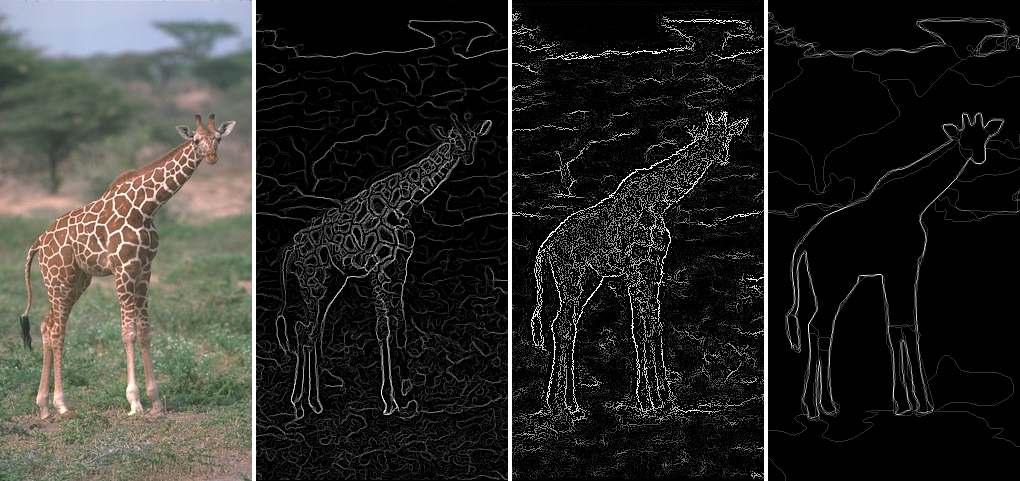
\includegraphics[width=0.8\textwidth]{graphics/canny.png}
    \caption{Example of edge detection \cite{nalwa_edge_1993}}
    \label{fig:edgedetection}
\end{figure}
%\subsubsection*{Point cloud}

%% Skoða hough transform...



% All edgel detectors seek to verify the existence of short linear edge segments that are postulated across image windows that have the same shape and size as the operator kernel. 


% skoða hough transform.
%% https://scholar.google.is/scholar?q=hough+transform+edge+detection&hl=en&as_sdt=0&as_vis=1&oi=scholart

%       \ifdraft{Hægt að sjá linka i links.tex}

%%%%%%%%%%%%%%%%%%%%%%%%%%%%%%%%%%%%%%%%%%%%%%%%%%%%%%%%%%%%%%%%%%
\subsubsection*{Convolutional neural network}
%\textbf{ÞARF AÐ BREYTA ÞESSUM kafla skoða comment fra martin}
% I think this chapter needs some more information about CNN:s (along with the appropriate references). What are they? How do the work? What does a typical CNN architecture look like? How many layers? What are the operations? What is the input? What is the output? etc.\textbf{It would be good to say something about why that is e.g. when using other machine learning methods like e.g. random forest you need to construct features}. 
In deep learning, a Convolutional Neural Network (ConvNet/CNN) is a class of deep neural network that is most applied to images, assign importance to various objects in the image, and differentiating one from the other. In CNN the pre-processing is much lower as compared to other classification algorithms. While the filters for primitive methods are man-made, ConvNets can learn these filters/filters with adequate training. CNN's advantages include that it can successfully capture the spatial and temporal dependencies in an image through the application of relevant filters. CNN was inspired by the organization of the visual cortex and the connectivity pattern of neurons in the human brain\cite{saha_comprehensive_2018}. 

In order to detect objects, recognize faces etc, CNNs use image recognition and classification. They consist of neurons with learning weights and preconditions. Each particular neuron received numerous inputs, then received a weighted sum, passed by an activation function and replied back with an output. CNNs are primarily used in the classification, grouping and recognition of objects by similarities. Many CNN algorithms can recognize the faces, road signs, animals, etc\cite{bansari_introduction_2019}.

\begin{figure}[h]
    \centering
    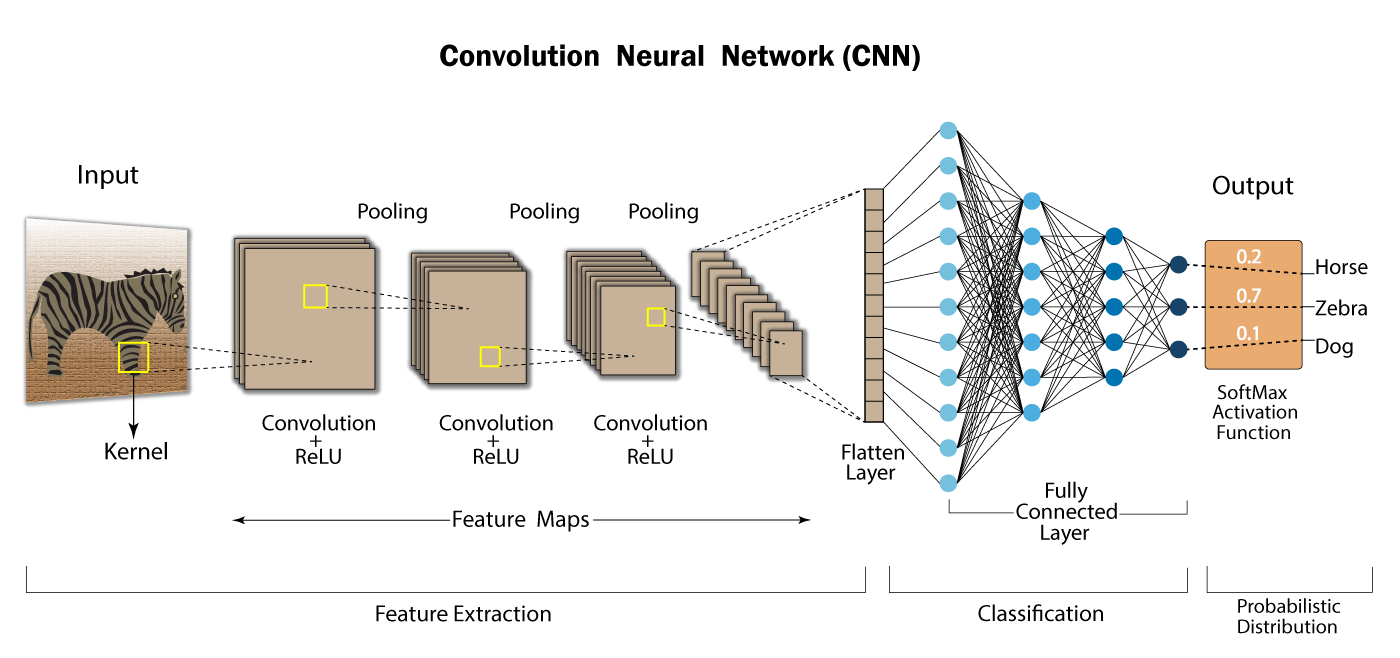
\includegraphics[width=1\textwidth]{graphics/methods/cnn.png}
    \caption{An example of how a CNN works\cite{e_convolutional_2020}}
    \label{fig:cnn}
\end{figure}

The CNN structure generally consists of two layers One feature is the extraction layer, each neuron input is connected to previous layers' local receptive fields, and the local feature is extracted. 
The position relation between this and other features will also be determined when the local features are extracted. The second is a map layer, and each network computer layer consists of a multi-function map. 
CNN is used primarily to indicate displacement, zoom and other distorting graphical invariance forms. 
Since the CNN functional detection layer learns by training data, explicit extraction of functionality is avoided, and training data are taught when using CNN implicitly\cite{liu_implementation_2015}. An example of how a CNN works and looks like in \textit{Figure \ref{fig:cnn}}




\subsubsection*{Object detection}
Object detection is an important task for computer vision that deals with the detection of instances of certain class objects in digital images (e.g. people, animals, or cars) an example is shown in \textit{Figure \ref{fig:mask}}. Object detection aims to develop models and techniques for computer vision that offer one of the most basic information necessary for computer vision applications\cite{zou_object_2019}. \textit{Where are these objects?}

\begin{figure}[h]
    \centering
    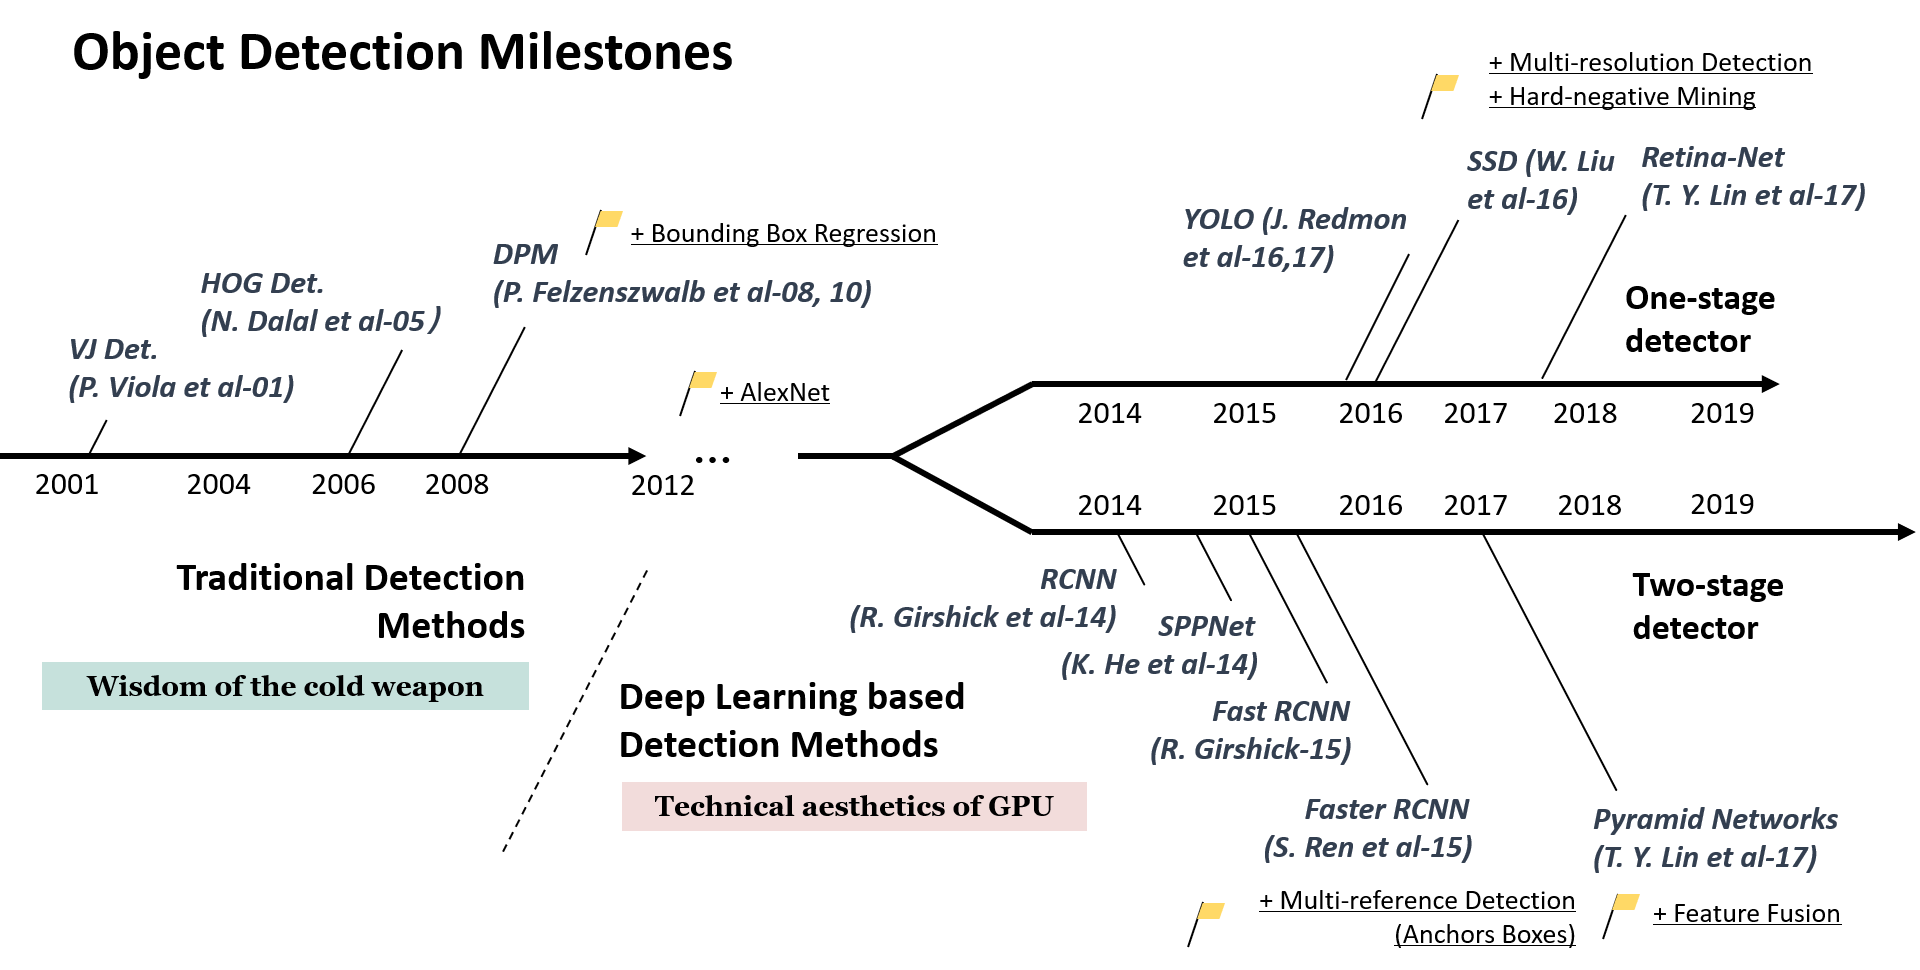
\includegraphics[width=0.9\textwidth]{graphics/objectdetection.png}
    \caption{Milestones in object detection \cite{zou_object_2019}}
    \label{fig:milestones}
\end{figure}
It has been widely accepted over the past two decades that the progress of object detection has usually been carried through two periods: the "traditional object detection (pre-2014)" and the "deep learning detection period" (post-2014). Milestones in object detections can be seen in \textit{Figure \ref{fig:milestones}}, in that figure it can be that there are many algorithms used for object detection. Some of the most commonly ones are \textit{Region-based Convolutional Neural Networks(R-CNN)}\cite{girshick_region-based_2016}, \textit{Fast R-CNN}\cite{girshick_fast_2015}, \textit{Faster R-CNN}\cite{ren_faster_2016}, \textit{Histogram of Oriented Gradients(HOG)}\cite{dalal_histograms_2005}, and \textit{You only look once(YOLO)}\cite{redmon_you_2016}.
%ÓKLÁRAÐ
\clearpage

% \subsection{Incremental Learning}
% \ifdraft{Hægt að sjá linka i links.tex}

%%%%%%%%%%%%%%%%%%%%%%%%%%%%%%%%%%%%%%%%%%%%%%%%%%%%%%%%%%%%%%%
\subsection{Robots}
Robots are getting smarter day by day and people wonder how much we can trust them in the industry. Collaborative Robots (Cobots) are more modern advances in which robots operate alongside humans rather than replacing them \cite{pickett_dont_2018}. 

Cobots assist operators by growing their capacities in terms of effort, enabling them to handle parts that are hot, heavy, bulky, or too fragile for precision handling. Besides, cobots are easier to program than industrial robots because they are capable of learning new jobs \cite{schmidbauer_teaching_2020}. A factory worker can easily re-program cobot, simply by moving his arm along the desired track. From there the cobot would learn the new movement and be able to replicate it on his own. Industrial robots can not be reprogrammed as easily and require the engineer to write a new code for any improvements in the process to be implemented.

Industrial automation is capable of achieving high productivity and repeatability in mass manufacturing. However, there is a lack of flexibility to overcome the uncertainties of workspaces arising from mass customization \cite{accorsi_application_2019}. Although humans can cope with such uncertainties and variability in such circumstances, their physical capacities are constrained in terms of repeatability, physical power, endurance, speed, etc. These constraints also lead to decreased performance and productivity. Therefore, a combination of automation and versatility is required to meet these overall manufacturing objectives through mass customization \cite{el_zaatari_cobot_2019}.   

\subsubsection*{Mathematical Robot Modeling:}
A mathematical representation must be built to generate trajectories and tasks for robots. This includes a model of the robot's geometry, mechanics, and electrical components. The mathematical model is developed to create a quantitative relationship between the sudden shift and the magnitude of the collision. The latter is represented by either an external impulsive force or an instantaneous change in the contact point's linear velocity. Second, as a result of the collision, large impulsive forces and constraint torques may develop within the system at each joint. These impulses can affect the system. A mathematical model is also established to create a quantitative relationship between the impulsive forces and torques of constraint and collision.  \cite{zheng_mathematical_1985}.

Robotic Manipulators are composed of two merged things, links, and joints that form a kinematic chain. In this context, links are the rigid sections that make up the mechanism and joints are the connection between two links. The kinematic manipulator chain is a combination of several cinematic pairs and the pair is a combination of two links connected by joint \cite{al-naimi_robotics_nodate}.

\begin{figure}[h]
    \centering
    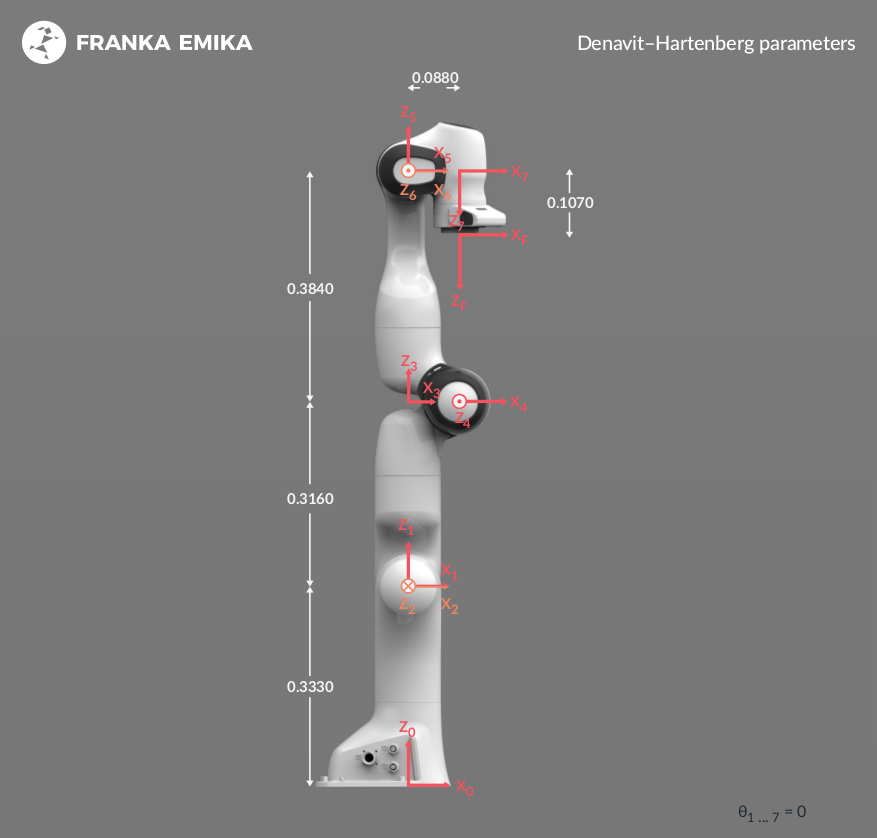
\includegraphics[width=0.7\textwidth]{graphics/pandakinematicchain.png}
    \caption{Panda’s kinematic chain \cite{noauthor_robot_nodate}}
    \label{fig:pandachain}
\end{figure}

\subsubsection*{Coordinate frame Transformations}
 %\url{https://www.maplesoft.com/content/EngineeringFundamentals/13/MapleDocument_13/Position,%20Orientation%20and%20Coordinate%20Transformations.pdf}
A 3D space pose or link has a 6 degree degree (DOF), translation\textit{(x,y,z)} and rotation $R \in SO(3)$. Depending on the application, the rotations may be expressed in several formats. 
In robotics, rotation matrices, rotations of the axis, quaternions and Euler angles are usually used to represent rotations.
A homogeneous matrix of transformation is a convenient way of bringing translations and rotations together to transform poses and coordinate frames\cite{cai_coordinate_2011}.

Three angles are the Euler angle of a rigid body which is introduced by Euler. Euler angles can describe the relative orientation between any two cartesian frames. After a rotation about the Z-axis, rotated Y-axis and the rotated X-axis(or the so-called 3–2–1) the Euler angles are adopted and move the reference frame into the frame. These three Euler angles are also referred to as the yaw (or heading), pitch, and roll angles\cite{cai_coordinate_2011}.

The three matrices of relative rotation are given by:
\begin{equation}
    R_{int1/nv} = R_{z}(\psi) = \begin{bmatrix}
cos(\psi)  & sin(\psi) & 0\\ 
-sin(\psi) & cos(\psi) & 0 \\ 
0 & 0 & 1
\end{bmatrix},
\end{equation}\label{eq:rz}

\begin{equation}
    R_{int2/int1} = = R_{y}(\theta) =  \begin{bmatrix}
cos(\theta)  & 0 & -sin(\theta)\\ 
0 & 1 & 0 \\ 
sin(\theta) & 0 & cos(\theta)
\end{bmatrix},
\end{equation}\label{eq:ry}
and 
\begin{equation}
    R_{b/int2} = R_{x}(\phi) =\begin{bmatrix}
1  & 0 & 0\\ 
0 & cos(\phi) & sin(\phi) \\ 
0 & -sin(\phi) & cos(\phi)
\end{bmatrix}.
\end{equation}\label{eq:rx}


For each angle axis, the Equations (\ref{eq:rz}), (\ref{eq:ry}) and (\ref{eq:rx})  show rotation matrices that can then be used for rotating around a fixed body or axis. An intrinsic rotation is a rotation on a body frame, whereas the external rotation is defined as an elemental rotation around a defined coordinate axis.
\begin{equation}
    R_{z(\psi)y(\theta)x(\phi)} = R_{z(\psi)} R_{z(\theta)}R_{x(\phi)}
\end{equation}
%Skoða
%\url{https://sci-hub.se/10.1007/978-0-85729-635-1_2} ... Þarf að skrifa úr þessu 


\subsection{Robot Operating System (ROS)}
Robot Operating System (ROS) is an open-source flexible framework for developing robot applications. It is a set of software, libraries, and conventions aimed at making the challenge of developing dynamic and robust robot actions over a wide range of robotic platforms easier. ROS is not a conventional operating system in the context of process control and scheduling \cite{quigley_ros_2009}. ROS offers package processing, message services between devices, and a variety of libraries. ROS supports a variety of programming languages, including C++, Python, and Javascript. ROS has over 3000 packages available, including robot drivers, computer vision libraries, navigation applications, and many more.
% \\
% \\ Það á eftir að skrifa þessa kafla hér :::::
% \textbf{Collision Detection:}
% \newline
% \textbf{Motion Planning:}
% \newline

\begin{figure}[h]%left, bottom, right and top
    \centering
    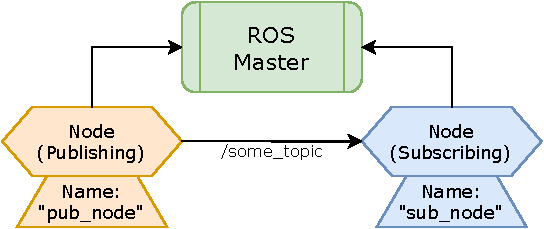
\includegraphics[width=0.8\textwidth]{graphics/rosmaster.pdf}
    \caption{This figure shows a basic ROS setup. The ROS master manages and establishes node connectivity. The correspondence is made by the subject /some\_topic in this example.}
    \label{fig:rosmaster}
\end{figure}

In a running ROS system, the \textbf{ROS Master} offers name and registration services to the other ROS nodes. It follows the topics and resources of the publishers and subscribers. The job of the master is to allow the location of individual ROS nodes. After these nodes are placed, they interact peer-to-peer\cite{noauthor_master_nodate}. An example of an ROS master can been seen in \textit{Figure \ref{fig:rosmaster}}.


\textbf{ROS nodes} are modules of the program which execute an operation. 
The nodes are autonomous and can be programmed in a programming language while also communicating in a different language with other nodes\cite{noauthor_rostutorialsunderstandingnodes_nodate}. An example of an ROS nodes can been seen in \textit{Figure \ref{fig:rosmaster}}.


The \textbf{ROS topics} are buses that exchange messages between nodes, implemented as named shared memory locations. Anonymous subjects have semantics publish/subscribe that decouple data output from consumption. Nodes are not generally aware of who they talk to. Instead, nodes interested in data subscribe to the subject concerned, and nodes that generate data publish to a specific topic. Many publishers and subscribers may participate in an issue\cite{noauthor_topics_nodate}. An example of an ROS topic can been seen in \textit{Figure \ref{fig:rosmaster}}.

A set of software packages integrated with the ROS and designed specifically to be aware of their surroundings and avoid collisions with humans and other obstacles is called \textbf{MoveIt!}. MoveIt! package implements solutions to the path planning problems that were mentioned in \textit{Section \ref{sec:binpicking}}. 
By using data fused from 3-D and other sensors, MoveIt! will allow robots to build up a representation of their environment. Also, generate motion plans that effectively and safely move the robot around in the environment, and execute the motion plans while constantly monitoring the environment for changes. 
%In other words, MoveIt! is an evolution arm navigation packages which were designed for motion planning and to create trajectories for simple paths with a single goal pose. 
MoveIt! provides a framework e.g., manipulation, kinematics, and motion planning. To calculate inverse and forward kinematics for path planning, and MoveIt packages uses Unified Robot Description Format(URDF). Configurations can then be created using the MoveIt set up assistant \cite{chitta_moveitros_2012}.

%------------------------------------
\section{Evaluation metrics}
\subsection{Intersection over union}
Intersection over Union (IoU) is known to be a good metric for overlapping two bounding boxes or masks and is used to measure object detector accuracy on a certain dataset. If the estimate is correct, then IoU = 1. The lower the IoU, the worse is the results \cite{sheremet_intersection_2020}.

\begin{figure}[h]
    \centering
    % include first image
    \subfloat[An example of a stop sign being detected in a picture. The prediction bounding box is red and the bounding box of the ground-truth is green. ]{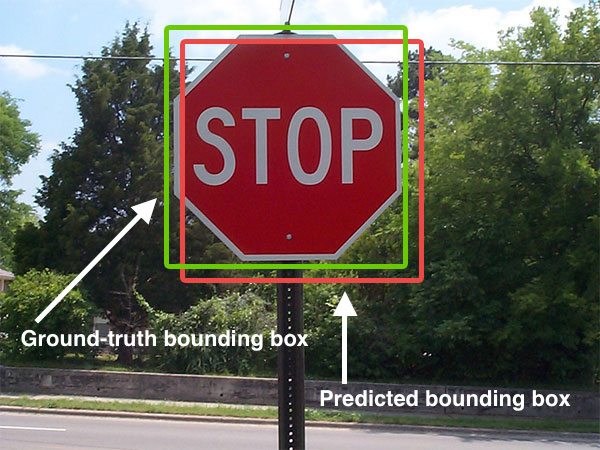
\includegraphics[width=0.48\textwidth]{graphics/iou_stop_sign.jpg}}
    \hfill
    \subfloat[The Intersection of Union are as simple as dividing the overlap zone between boundaries by the union area]{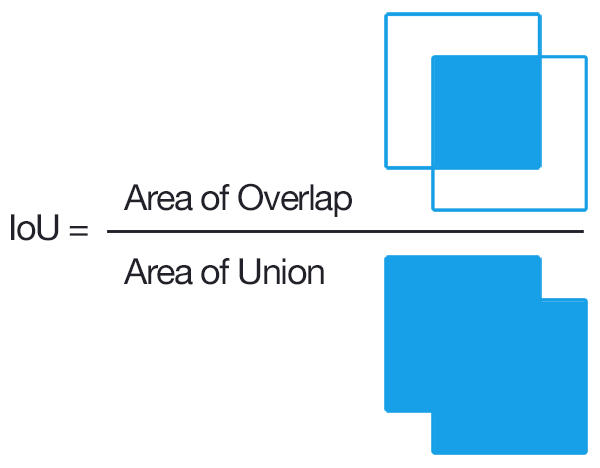
\includegraphics[width=0.48\textwidth]{graphics/iou_equation.png}\label{figure: ioueq}}
    \caption{Intersection over Union for object detection \cite{rosebrock_intersection_2016}}
    \label{figure: iou}
\end{figure}

\begin{equation}
    IoU = \frac{Area\ of\ Overlap}{Area\ of\ Union} \label{eq: ioueq}
\end{equation}
\vspace{0.5cm}

Intersection over Union is simply a ratio between the area of overlap and area of the union when looking at \textit{Equation \ref{eq: ioueq}}.
In the numerator, the area of overlap is calculated between the predicted bounding box and the bounding box.
The denominator is the area of union or, rather, the area covered by both the foreseen boundary and the bottom-wheel boundary\cite{uavs_comparing_2019}.
%\vspace{1cm}
\subsection{Recall, Precision, and F1}
When tests of the performance on the retrieval systems were first developed, an empirical tendency was noticed for recall (completeness) and accuracy (cleanliness of retrieval), both of which appeared to be inversely connected\cite{buckland_relationship_1994}. \textit{Figure \ref{fig:precisionrecall}} explains the precision and recall.



\begin{itemize}
    \item True Positive (TP): The actual positive class is predicted positive.
    \item True Negative (TN): The actual negative class is predicted negative.
    \item False Positive (FP): The actual class is negative but the predicted class is Positive
    \item False Negative (FN): The actual class is positive but the predicted class is negative.
\end{itemize}

\begin{figure}[h]
    \centering
    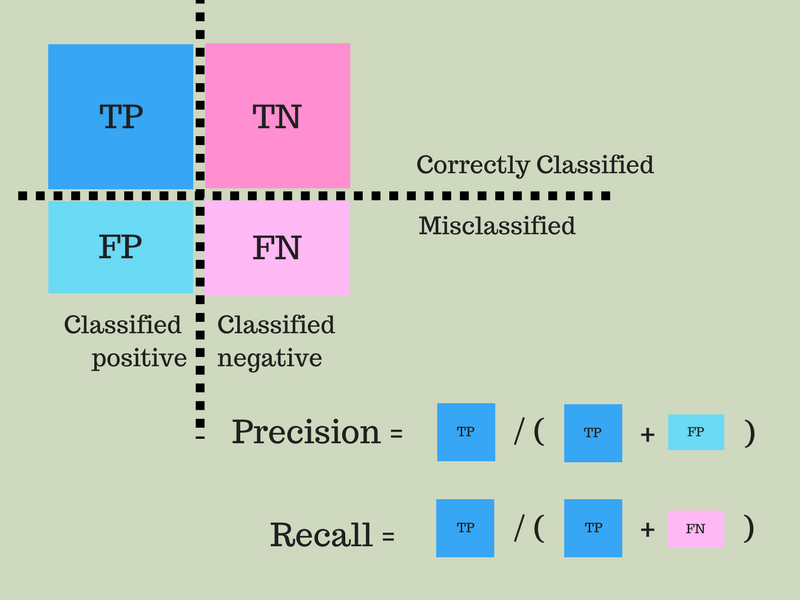
\includegraphics[width=0.8\textwidth]{graphics/Precisionrecall.png}
    \caption{Precision and recall explained \cite{mittapally_whats_2019}}
    \label{fig:precisionrecall}
\end{figure}



Precision is the ratio between the True Positives and all the Positives. In this project, the precision was measured by the number of bottles that were correctly identify out of all the bottles in the bin. It can bee seen in \textit{Equation \ref{eq:precision}}. Precision shows a measure of relevant data points\cite{shung_accuracy_2020}.
\begin{equation}
    Precision = \frac{True\ Positive(TP)}{True\ Positive(TP)+False \ Positive(FP)}
    \label{eq:precision}
\end{equation}


The recall is the measurement of the model that identifies true positives properly. Recall calculates the number of the correct detections divided by the number of actual detections\cite{shung_accuracy_2020}. Recall quantifies the number of positive class predictions made out of all positive examples in the dataset. An example of how recall is calculated can be seen in \textit{Equation \ref{eq:recall}}.
\begin{equation}
    Recall = \frac{True\ Positive(TP)}{True\ Positive(TP)+False \ Negative(FN)}
    \label{eq:recall}
\end{equation}

The F-score is a measure of the precision of a model on a dataset. This evaluation is done to evaluate binary classification systems, classifying examples into positive or negative classification systems. 
The F-score combined the precision and recall of the model and is described as the harmonic mean to the precision and recall of the model\cite{wood_f-score_2019}.
An example of how F-score is calculated can be seen in \textit{Equation \ref{eq:f1score}}.
\begin{equation}
    F- score = F_1 = 2 \cdot \frac{Precision \cdot Recall}{Precision + Recall}
    \label{eq:f1score}
\end{equation}


\section{Objectives}
The objective of this project was to answer the following research questions:
\begin{enumerate}[i.]
    \item Is it possible to generate new arrangements of objects using a robot manipulator?
    \item Is it possible to annotate objects automatically,  determining the extent of the objects in the images?
    \item Is it possible to improve the performance of a Convolutional Neural Network using automatically generated training data from robot? %How will the accuracy of object detection be, using a deep neural network trained on the robot-generated data?
\end{enumerate}